\begin{frame}
  \frametitle{Empirical questions}

  \begin{itemize}

  \item How much data is needed for R-W learning convergence with the
    Danks equilibria

  \item Are there cases where we observe non-convergence between the
      R-W learning associations and Danks equilibria -- if yes, why?

    \item Does NDL accuracy always improve with increasing cues?
      If not, why?
      
  \end{itemize}
  
\end{frame}

\begin{frame}
  \frametitle{Non-equivocal positive assocation -- convergence}

  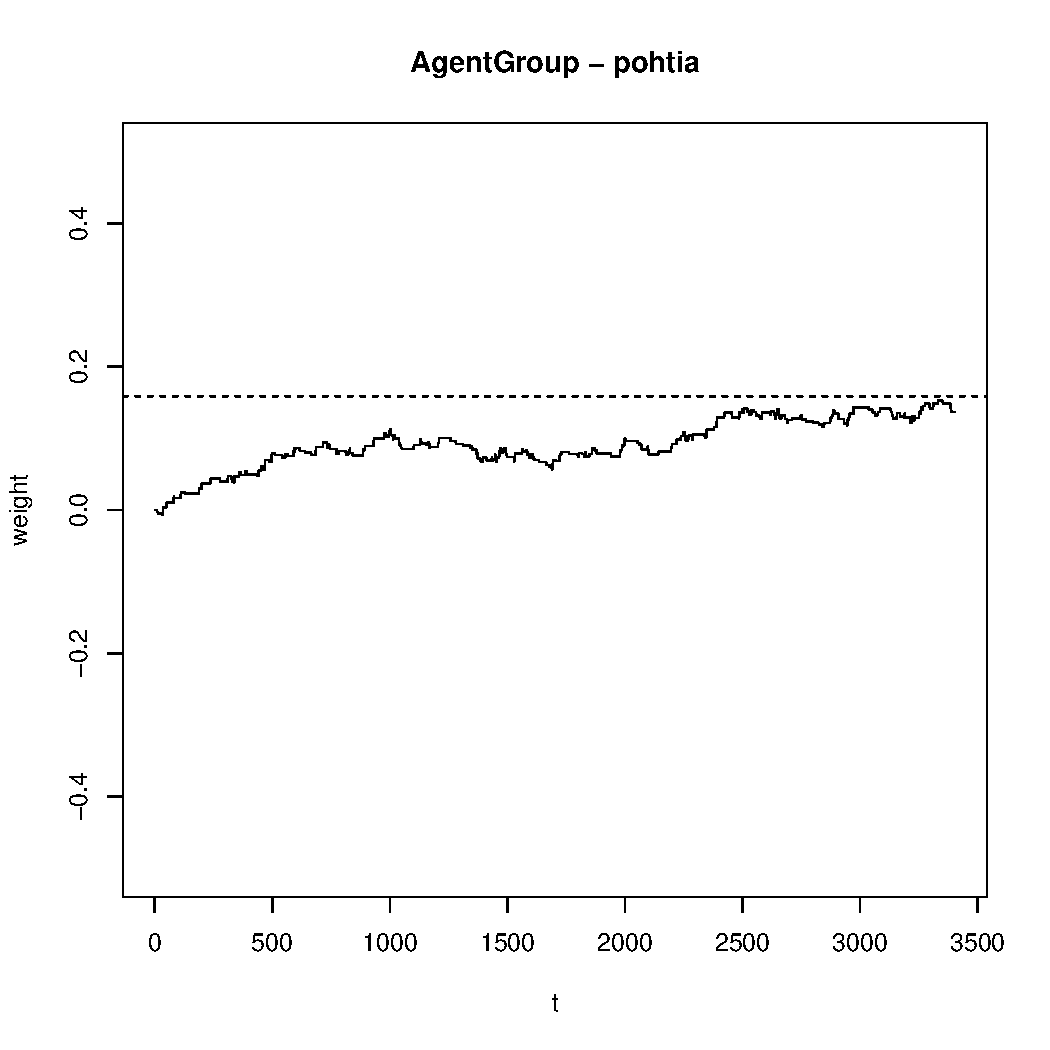
\includegraphics[width=8cm]{{{img/think.qitl2.AgentGroup_pohtia_RW_vs_D}}}

\end{frame}

\begin{frame}
  \frametitle{Non-equivocal positive association -- convergence with 1x data}

  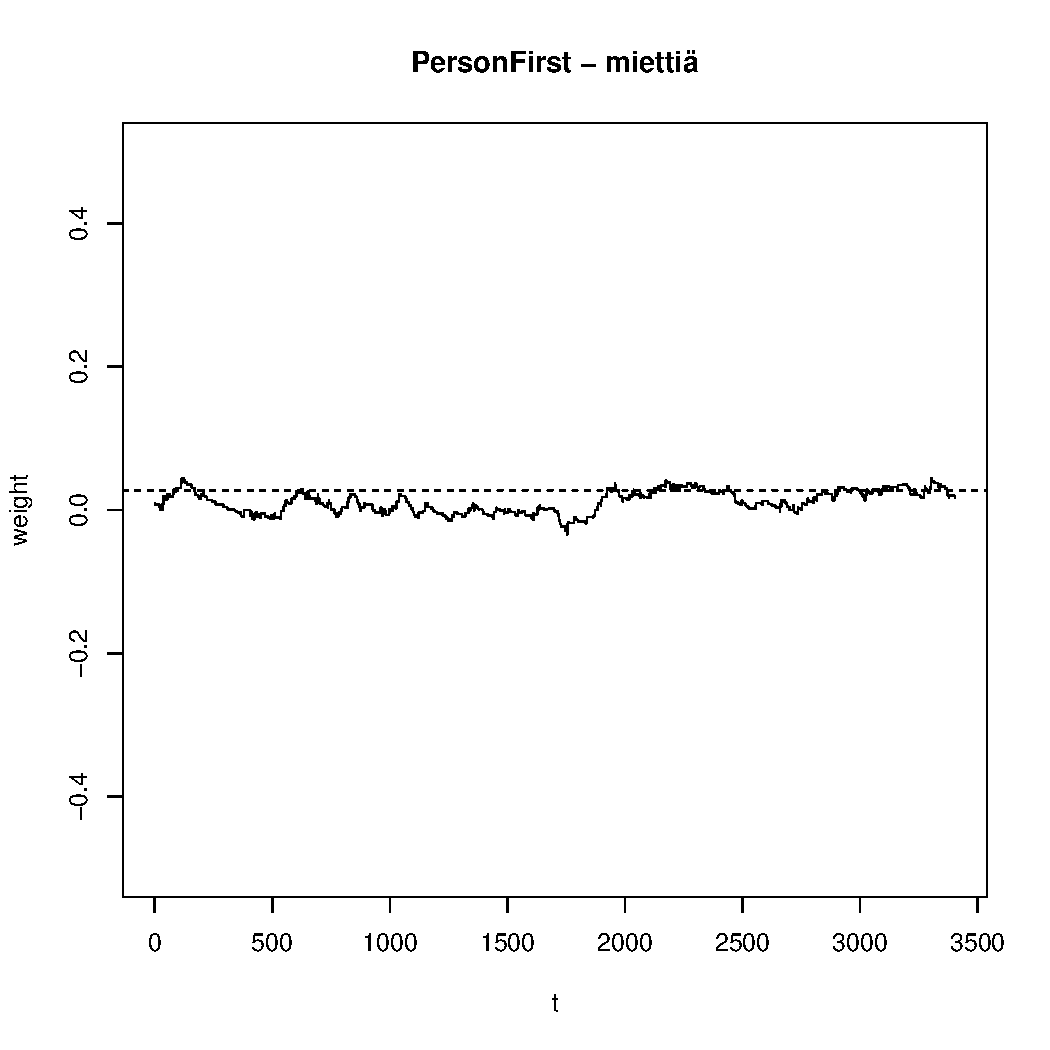
\includegraphics[width=8cm]{{{img/think.qitl2.PersonFirst_miettia_RW_vs_D}}}

\end{frame}

\begin{frame}
  \frametitle{Non-equivocal negative association -- convergence with 1x data}

  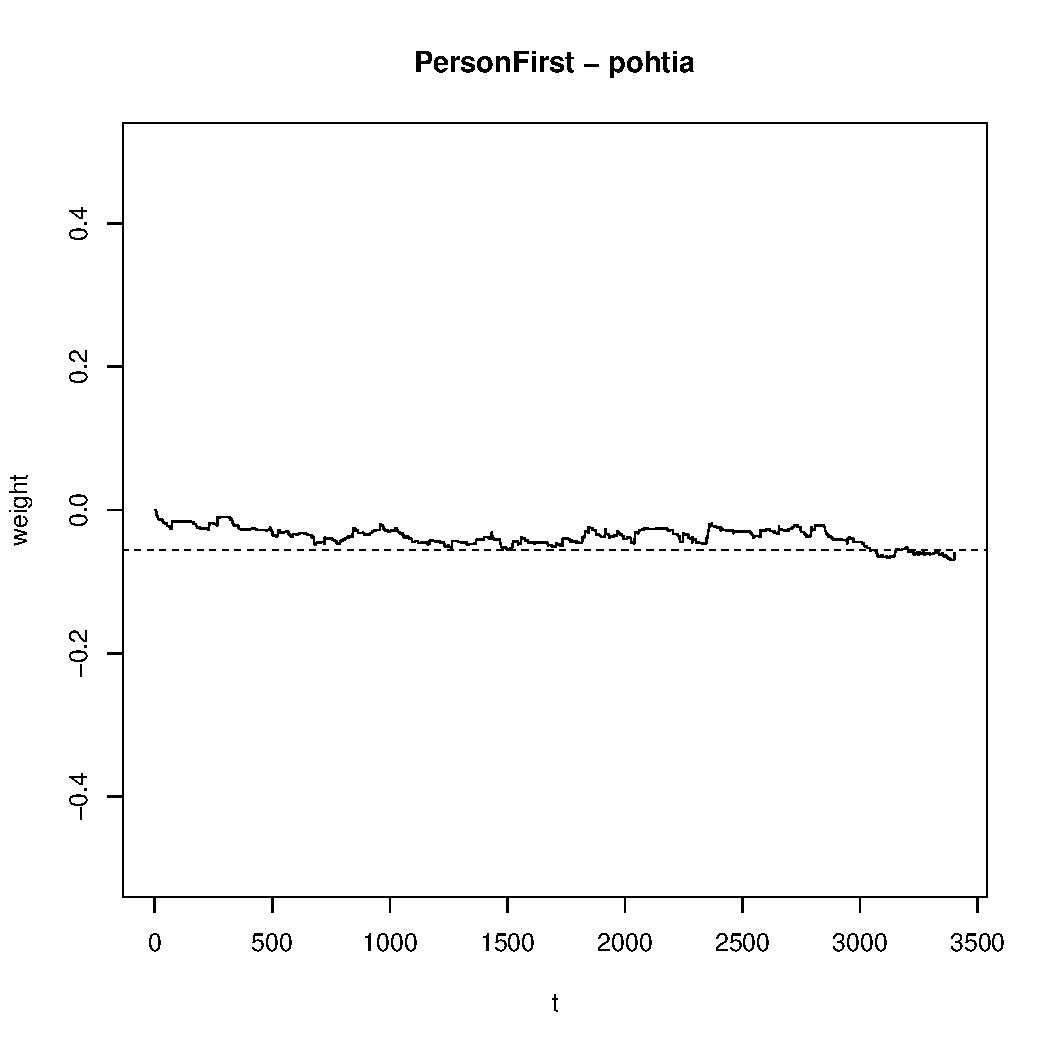
\includegraphics[width=8cm]{{{img/think.qitl2.PersonFirst_pohtia_RW_vs_D}}}

\end{frame}

\begin{frame}
  \frametitle{Near-perfect positive association -- non-convergence with 1x data}

  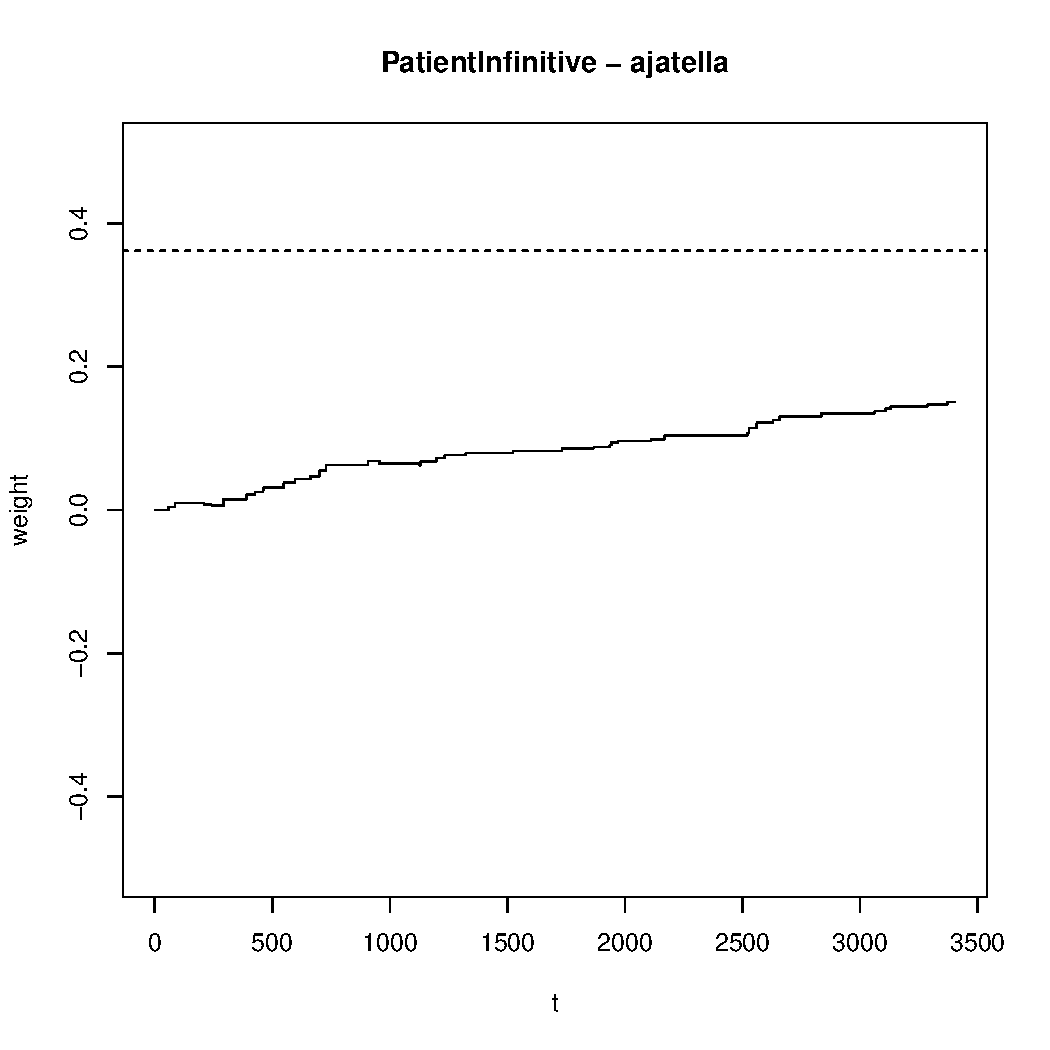
\includegraphics[width=8cm]{{{img/think.qitl2.PatientInfinitive_ajatella_RW_vs_D}}}

\end{frame}

\begin{frame}
  \frametitle{Near-perfect negative association -- non-convergence with 1x data}

  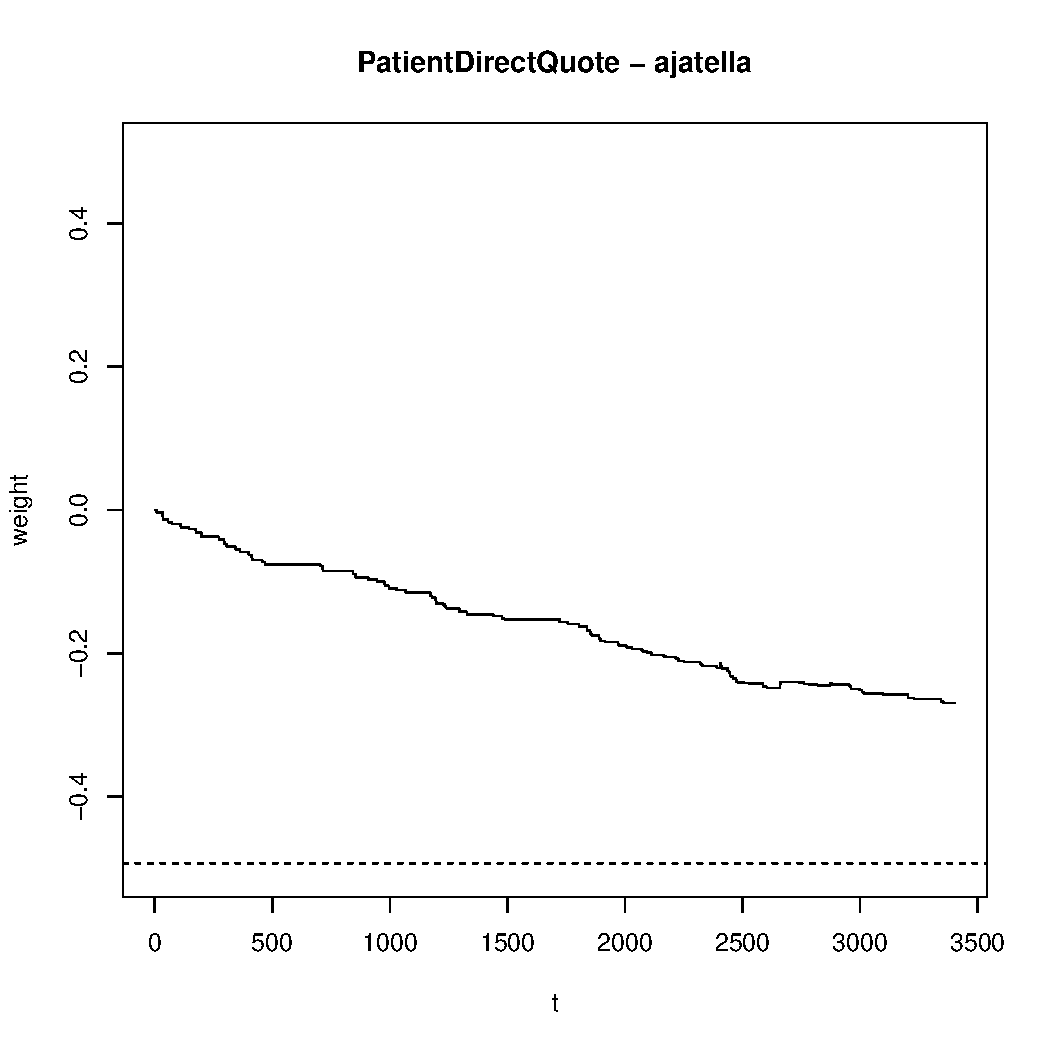
\includegraphics[width=8cm]{{{img/think.qitl2.PatientDirectQuote_ajatella_RW_vs_D}}}

\end{frame}

\begin{frame}
  \frametitle{Near-perfect positive association -- convergence with 5x data}

  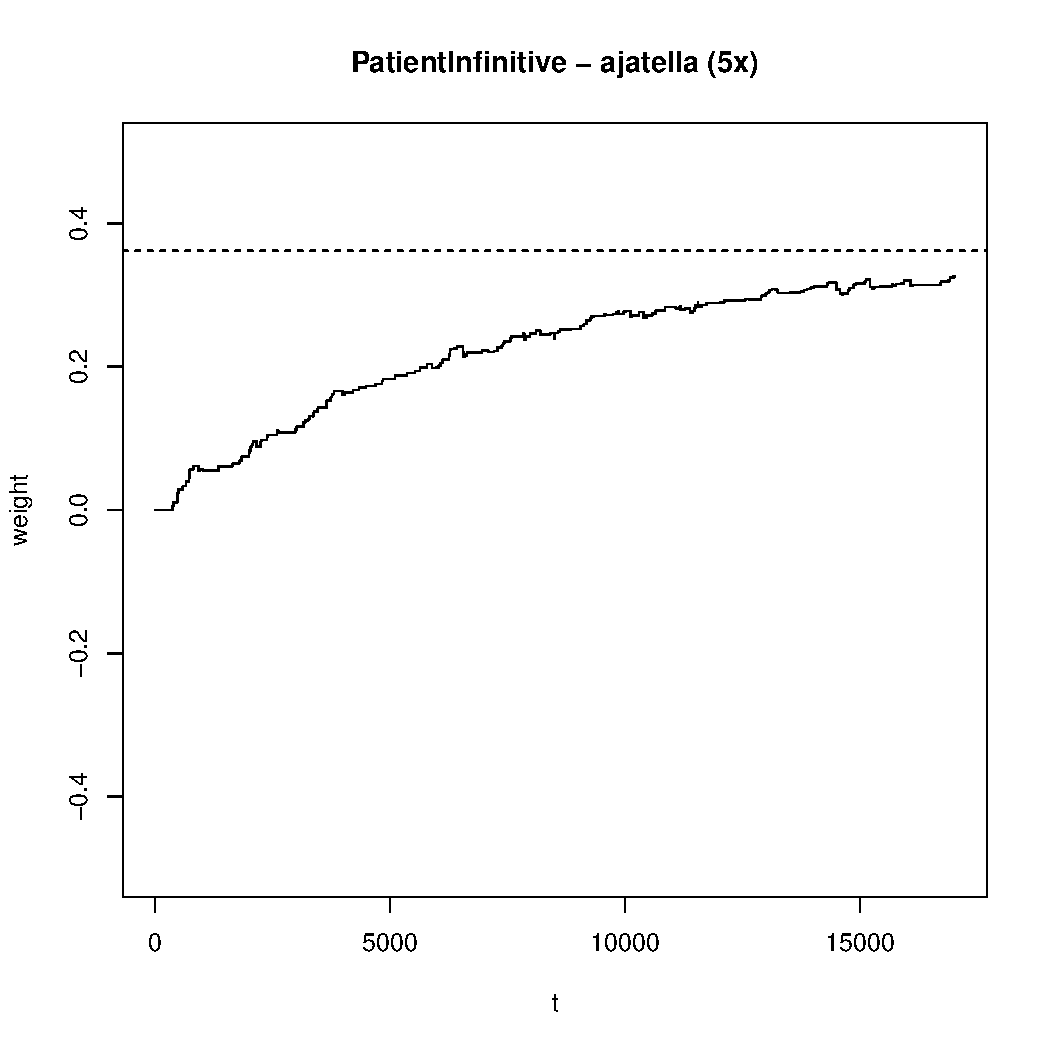
\includegraphics[width=8cm]{{{img/think.qitl2.PatientInfinitive_ajatella_RW_vs_Dx5}}}

\end{frame}
\begin{frame}
  \frametitle{Near-perfect negative association -- convergence with 5x data}

  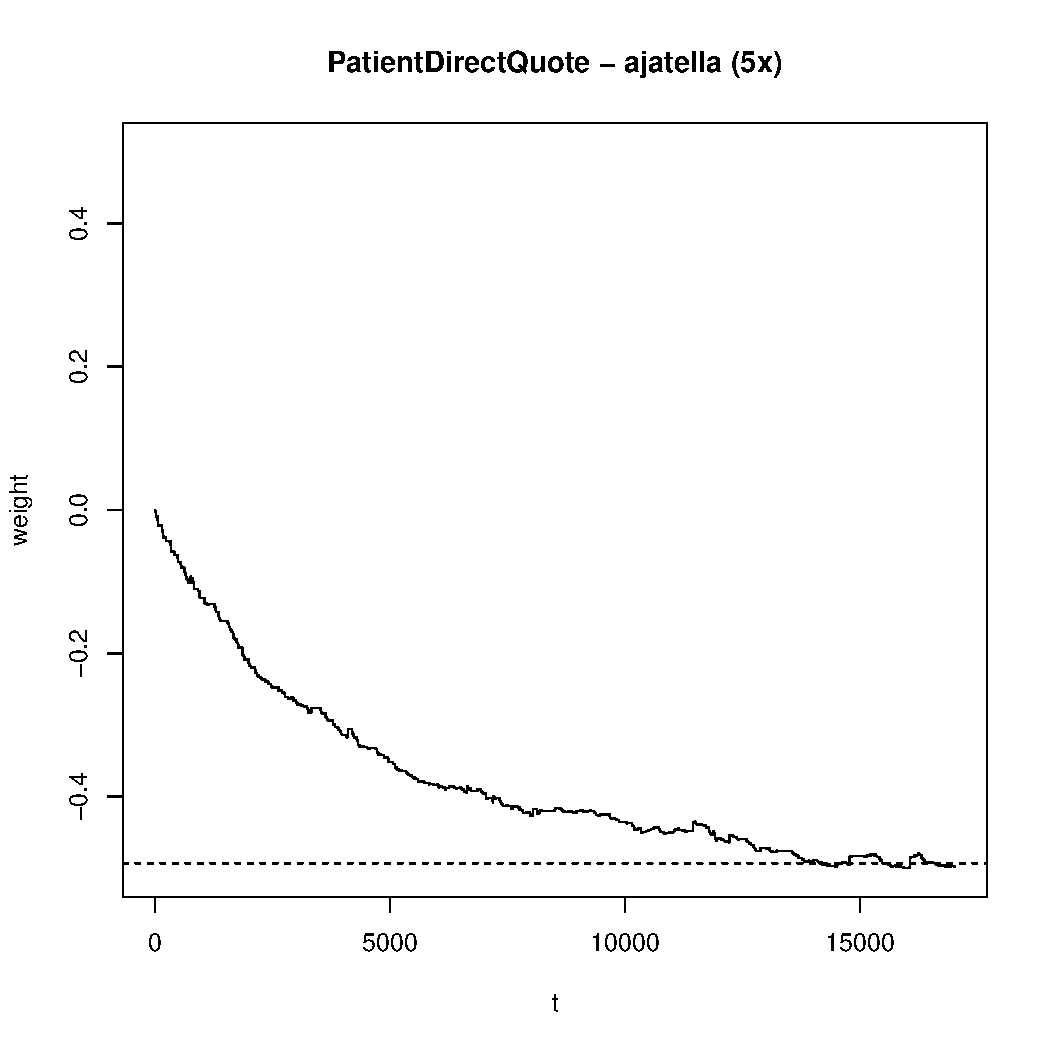
\includegraphics[width=8cm]{{{img/think.qitl2.PatientDirectQuote_ajatella_RW_vs_Dx5}}}

\end{frame}
  
%%% Local Variables: 
%%% mode: latex
%%% TeX-master: "../qitl6_evert_arppe"
%%% End: 
